% Формат бумаги: А4.
\documentclass[a4paper]{report}

% UTF-8 encoding
\usepackage[utf8]{inputenc}
% Russian
\usepackage[english,russian]{babel}

\usepackage{amsmath,amsfonts,amssymb,cite,url,verbatim,graphicx,wrapfig,physics,seqsplit}

\usepackage{bm,mathrsfs}
\usepackage{smartdiagram}

% Подрисунки
\usepackage{subfigure}
\usepackage[subfigure]{tocloft}

\usepackage{booktabs}
\graphicspath{{images/}}
\DeclareGraphicsExtensions{.pdf,.png,.jpg}

% Поля: верхнее – 2 см, нижнее – 2 см, левое – 3 см, правое – 1.5 см.
%\usepackage[showframe]{geometry} % showframe - показать рамки
\usepackage{geometry}
\geometry{
	left = 3cm,
	top = 2cm,
	right = 1.5cm,
	bottom = 2cm
}


\usepackage{listings}

% Кегль:
%% текст в таблице, подписи к рисункам, таблицам – 12 пт,
\renewcommand{\small}{\fontsize{12}{12}\selectfont}
%% основной текст – 14 пт,
\renewcommand{\normalsize}{\fontsize{14}{14}\selectfont}
%% названия параграфов – 16 пт,
\renewcommand{\large}{\fontsize{16}{16}\selectfont}
%% названия глав – 18 пт,
\renewcommand{\Large}{\fontsize{18}{18}\selectfont}
\renewcommand{\Huge}{\fontsize{20}{20}\selectfont}


\usepackage{sectsty}
\sectionfont{\Large}
\subsectionfont{\large}
\paragraphfont{\normalsize}
\usepackage[font=small]{caption}

% Межстрочный интервал: 1.5 строки.
\linespread{1.5}

% Абзацный отступ. Первая строка каждого абзаца должна иметь абзацный отступ 1.25 см.
\usepackage{indentfirst}
\setlength{\parindent}{1.25cm}

% Выравнивание основного текста по ширине поля.
\usepackage{ragged2e}
\justifying

% Отключение расстановки переносов + нормальная ширина строки
\pretolerance=1000
\hyphenpenalty=10000
\tolerance=2000 
\emergencystretch=25pt

%%% здесь лучше ничего не трогать
% Глубина: 1=глава-раздел
\setcounter{tocdepth}{1}

% Выключение нумерации раздела
%\renewcommand{\thesection}{}
% Выключение нумерации подраздела
%\renewcommand{\thesubsection}{}

% Выравниваение параграфов (разделов) по центру
\allsectionsfont{\centering}

\usepackage{titlesec}
\usepackage{titletoc}% http://ctan.org/pkg/titletoc
% Какая-то команда
%\newcommand{\sectionbreak}{\clearpage}

%\cftsetindents{chapter}{0em}{0em}
%\cftsetindents{subsection}{2em}{0em}
% Какие-то отступы
%\cftsetindents{section}{0em}{0em}
%\cftsetindents{subsection}{2em}{0em}


% Настройка отображения главы в тексте
\titleformat{\chapter}[display]
	{\filcenter}
	{\bfseries \Large{\chaptertitlename~\thechapter}}
	{15pt}
	{\bfseries \Large}{}

% Настройка вертикальных и горизонтальных отступов
\titlespacing*{\chapter}{0pt}{0pt}{8pt}
\titlespacing*{\section}{\parindent}{*4}{*4}

% Название для оглавления с отступом после него на 2,5 см
\AtBeginDocument{\renewcommand{\contentsname}{\begin{center} \vskip-2.5cm \Large{Содержание}\end{center}}}
\AtBeginDocument{\renewcommand{\bibname}{}}

% Настройка отображения главы в содержании
\titlecontents{chapter}% <section-type>
	[0pt]% <left>
	{}% <above-code>
	{\bfseries\chaptername~\thecontentslabel.~}% <numbered-entry-format>
	{}% <numberless-entry-format>
	{\bfseries\titlerule*[1pc]{.}\contentspage}% <filler-page-format>

% Настройка отображения раздела в содержании	
\titlecontents{section}% <section-type>
	[1.25cm]% <left>
	{}% <above-code>
	{\thecontentslabel~}% <numbered-entry-format>
	{}% <numberless-entry-format>
	{\titlerule*[1pc]{.}\contentspage}% <filler-page-format>
	
% Точка в номере параграфа и значок параграфа
%\renewcommand{\thesection}{\S~\arabic{chapter}.\arabic{section}.}

% Сброс нумерации формул, рисунков, таблиц
%\renewcommand{\theequation}{\arabic{equation}}
\usepackage{chngcntr}
\counterwithout{equation}{chapter}
\counterwithout{figure}{chapter}
\counterwithout{table}{chapter}

% Установка шрифтов
\usepackage{sectsty}
\chapterfont{\Large}
\sectionfont{\large\centering}
\paragraphfont{\normalsize}
\usepackage[font=small]{caption}

%%%
\newtheorem{teor}{Теорема}
\newtheorem{defin}{Определение}

% Точка вместо двоеточия в названиях рисунков и таблиц
\usepackage[labelsep=period]{caption}

% Цвет текста
\usepackage{xcolor}

% Clicable TOC
\usepackage{hyperref}
\hypersetup{
	colorlinks,
	citecolor=black,
	filecolor=black,
	linkcolor=black,
	urlcolor=black
}

% Список литературы, убрать лишнюю страницу
\usepackage{etoolbox}
\patchcmd{\thebibliography}{\chapter*{\bibname}}{\section*{\bibname}}{}{}

% This pack­age gives you easy ac­cess to the Lorem Ip­sum dummy text; an op­tion is avail­able to sep­a­rate the para­graphs of the dummy text into TEX-para­graphs.
\usepackage{lipsum}



%Tikz Pictures
\usepackage{tikz}
\usetikzlibrary{arrows,decorations.pathmorphing,backgrounds,positioning,fit,petri}
\usetikzlibrary{arrows,shapes,backgrounds,calc,positioning}
\usetikzlibrary{mindmap}
\graphicspath{{images/}}

\usepackage{smartdiagram}
\usesmartdiagramlibrary{additions}



\usepackage{pythonhighlight}


\begin{document}
	\thispagestyle{empty}
	\begin{center}
		\textsc{Санкт-Петербургский государственный университет \\
			\textbf{Кафедра математической теории игр и статистических решений}} \\
		\vspace{2cm}
		\Large{\textbf{Зуенок Кристина Владимировна}} \\
		\vspace{2cm}
		\large{\textbf{Выпускная квалификационная работа бакалавра}} \\
		\vspace{1cm}
		\Large{\textbf{Об исследовании доли ВИЧ-инфицированных среди некоторых групп населения}} \\
		\normalsize{Направление 02.03.02 \\
			Фундаментальная информатика и информационные технологии} \\
	\end{center}
	\vspace{2cm}
	\hspace{9cm} Научный руководитель, \\
	\hspace*{9cm} доктор физ.-мат. наук, \\
	\hspace*{9cm} доцент \\
	\hspace*{9cm} Громова Е. В.\\
	\begin{center}
		\vfill
		Санкт-Петербург \\
		2018
	\end{center}
	\newpage
	%%%%% CONTENTS %%%%%
	\tableofcontents
	\newpage
	
	\chapter*{Введение}
	\addcontentsline{toc}{chapter}{\bfseries Введение}
	
	Со времени начала глобальной пандемии ВИЧ/СПИДа в начале 1980-х годов около 70 миллионов человек были инфицированы и 35 миллионов умерли от болезней, связанных со СПИДом \cite{link1}. В связи с этим, распространение ВИЧ и СПИД на протяжении многих лет является предметом различных теоретических и медицинских исследований \cite{link2}. 
	
	Актуальными проблемами общественного здравоохранения является сбор информации, ее анализ для оценки текущей ситуации и оптимальное распределение ограниченных ресурсов между различными программами лечения и профилактики. 
	Чем больше информации становится известно о ВИЧ, тем сложнее становятся математические модели, разрабатываемые для контроля распространения заболевания. 
	
	Последние достижения в области профилактики ВИЧ демонстрируют новые формы высокоактивной антиретровирусной терапии (ВААРТ), ставшие настолько эффективными, что вирусная нагрузка у инфицированных пациентов становится необнаруживаемой, и пациенты по существу не способны заразить других людей. Альтернативой является использование новых методов предэкспозиционной или доконтактной профилактики ВИЧ, нацеленной на неинфицированных людей, снижающие вероятность заражения вирусом даже при частых контактах.
	
	Однако, даже имея в распоряжении методы лечения, эффективные для блокировки передачи вируса от инфицированных лиц, а также для защиты неинфицированных лиц от заражения, все еще сложно однозначно ответить, как именно данные инновации должны быть применены.
	
	Основным препятствием является то, что, хотя эффективность этих вмешательств на индивидуальном уровне может быть определена с помощью контролируемых испытаний, их эффективность для общественного здравоохранения не может быть установлена однозначно. Это связано с тем, что популяции отличаются друг от друга как динамикой передачи ВИЧ, так и доступностью ресурсов для профилактики.
	
	
	Вместе с такой постановкой проблемы возникает другая - сложность оценки соотношения людей в популяции, которым необходима та или иная терапия. Для отражения реальной ситуации, рассматриваемой в исследовании, выборка должна быть репрезентативной, то есть представлять генеральную совокупность - все население - наиболее полно, отражая настоящее соотношение входящих в нее групп.	
	\begin{comment}
	 Мерой репрезентативности выборки является ее ошибка - расхождение между двумя совокупностями — генеральной, на которую направлен теоретический интерес социолога и представление о свойствах которой он хочет получить в конечном итоге, и выборочной, на которую направлен практический интерес, которая выступает одновременно как объект обследования и средство получения информации о генеральной совокупности.
	На практике ошибка репрезентативности определяется путем сравнения известных характеристик генеральной совокупности с выборочными средними. В социологии при обследованиях взрослого населения чаще всего используют данные переписей населения, текущего статистического учета, результаты предшествующих опросов. В качестве контрольных параметров обычно применяются социально-демографические признаки. Сравнение средних генеральной и выборочной совокупностей, на основе этого определение ошибки выборки и ее уменьшение называется контролированием репрезентативности.
	\end{comment}
	Если выборочная совокупность составлена правильно, то результаты, характеризующие всю генеральную совокупность, считаются надежными, иначе, при недостаточном объеме выборки или существенном смещении, ценность проведенного исследования значительно снижается.

	
	\begin{comment}	
	Прежде всего на основе имеющихся данных необходима оценка соотношения людей в популяции, которым необходима та или иная терапия. 
	Итак, определение плана действий сектора здравоохранения по борьбе с ВИЧ, т.е. оптимальной стратегии распределения ограниченных ресурсов, невозможно без учета следующего: 
	\end{comment}
	
	Вне всяких сомнений, решение вышеупомянутых проблем должно основываться на модели основополагающих медицинских, биологических и социальных процессов, отражающих соответствующие особенности населения. 
	
	Данная работа рассматривает динамическую эпидемиологическую модель. Предполагается, что целевая популяция состоит из популяции МСМ ограниченной географической единицы (т.е. крупного города, региона или страны), демонстрирующей два разных уровня рискованного поведения. Кроме того, рассматриваются две разные стадии заболевания, острая и хроническая, так как острая стадия связана со значительно более высокой инфекционностью. Данные, доступные для исследования, формируются на основе опросов и тестов, полученных в некоторой высокорисковой среде, и представляют собой нерепрезентативную выборку.

	
	
	\chapter*{Постановка задачи}
	\addcontentsline{toc}{chapter}{\bfseries Постановка задачи}
	
	В работе рассматривается эпидемиологическая модель, описывающая население, которое может быть поделено на несколько различных между собой групп с соответствующими состояниями, основываясь на разнохарактерном поведении индивидов и их ВИЧ-статусе.
	При этом между состояниями осуществляются переходы в связи с инфицированием людей, сменой поведения и иными причинами, рассмотренными далее.
	
	Формальная постановка задачи может быть представлена следующим образом: пусть существует некоторая популяция $P$, имеющая размер $N = |P|$, из которой производят выборку $S$ при дополнительных условиях отбора, нарушающих ее репрезентативность, объемом $N_S = |P|$, $S \subset P$.
	
	Необходимо разделить рассматриваемое население $P$ на возможные категории: $S_{(\cdot)}$, $I_{(\cdot \cdot)}$.
	
	Сформулировать и проанализировать математическую модель, учесть возможное взаимодействие между группами индивидов, развитие, приток новых исследуемых $ \alpha_{(\cdot)}$ и их отток $\mu$ из системы.
	
	Оценить доли здоровых $s_{(\cdot)}$ и ВИЧ-инфицированных $i_{(\cdot \cdot)}$ людей из различных категорий во всей популяции $P$, на основании данных о заболеваемости $\hat{s}_{(\cdot)}$ и $\hat{i}_{(\cdot \cdot)}$ в некоторой выборке $S$ (в частности, данных, полученных при тестировании отдельных индивидов в рамках исследования) в условиях нерепрезентативности выборки.
	
	Оценить количество людей в различных состояниях $S_{(\cdot)}$, $I_{(\cdot \cdot)}$ для всей популяции $P$.
	Осуществить программную реализацию модели и анализ полученных результатов.

	
	
	\chapter*{Обзор литературы}
	\addcontentsline{toc}{chapter}{\bfseries Обзор литературы}
	
	Одной из первых работ, посвященных моделированию процессов, связанных с ВИЧ, является статья \cite{link3}, представляющая численное моделирование нескольких процессов, которые учитывают такие факторы, как переменная инфекционность индивидов и переменные инкубационные периоды в гомосексуальной среде.
	Оценка поведения индивидов была учтена в работе \cite{link4}, где Андерсон представил модель распространения заболевания среди гомосексуального населения Великобритании, используя реальные данные, и рассмотрел последствия изменений в сексуальном поведении. В последующих работах \cite{link5, link6} Андерсон и его коллеги в продолжение исследований проанализировали модель распространения ВИЧ в гетеросексуальных сообществах в развивающихся странах и изучили влияние стратегий контроля.
	 
	Хотя большинство случаев ВИЧ-заболеваний в развитых странах происходят в гомосексуальном обществе, болезнь распространяется на гетеросексуальное общество. Хеткотт \cite{link7} представил общую модель, которая объясняет взаимодействие между индивидами с различной сексуальной ориентацией и потребителями инъекционных наркотиков.
	
	Несмотря на снижение во всем мире ежегодного числа новых случаев заболеваемости ВИЧ, среди мужчин, имеющих половые контакты с мужчинами (МСМ) в развитых странах заболеваемость увеличивается \cite{link8, link9}. Термин МСМ был впервые употреблен в 1990-х годах и используется в эпидемиологии и социальных исследованиях для обозначения мужчин, постоянно или переодически практикующих сексуальные контакты с другими мужчинами. При этом сексуальная ориентация и сексуальная идентичность не принимаются во внимание \cite{link10}. Значительную часть МСМ составляют бисексуальные мужчины и даже состоящие в гетероксуальном браке, также категория включается в себя лиц мужского пола, идентифицирующих себя как женщин \cite{link11}.
	По данным UNAIDS \cite{link12}, МСМ находятся на пятом месте по распространенности ВИЧ (после потребителей инъекционных наркотиков, их партнеров, работников сферы секс-услуг и их партнеров) в мире среди людей с рискованным поведением. Однако в конкретных странах ситуация совершенно иная. Например, в Северной Америке, Австралии, Новой Зеландии и большинстве стран Западной Европы почти 70\% всех новых случаев заражения ВИЧ приходится на МСМ \cite{link13}. В Канаде - 40\%. В США в 2013 году 65\% новых случаев заражения ВИЧ также связано с МСМ \cite{link14}.
	
	Согласно исследованиям, менее 5\% всех мужчин, относящихся к категории МСМ, имеют доступ к услугам по профилактике и уходу в связи с ВИЧ, в которых они нуждаются. Этому способствуют различные факторы, в частности, низкий уровень информированности о ВИЧ и о рискованном сексуальном поведении, гомофобия, социальная стигматизация и дискриминация МСМ, в том числе и со стороны медицинских работников \cite{link15}.
	
	В статье \cite{link16} приводится анализ роста ВИЧ в упрощенной версии модели, представленной Хайманом и Стэнли \cite{link3} для МСМ-сообщества, в которой учитывается непропорциональное смешивание различных групп риска. Из-за упрощающих допущений, которые используют авторы, модель не может дать точные прогнозы распространения ВИЧ-инфекции. Однако простая форма модели отражает большую часть качественного поведения более сложных моделей и позволяет количественно анализировать распространение инфекции через различные группы риска и исследовать динамику распространения из одной группы риска в другую.
	
	Одной из важнейших работ, рассматривающих моделирование ВИЧ-инфекции является статья \cite{link17}, опубликованная в 1989 году.
	Особенностью работы стало использование байесовского подхода для включения в модели неопределенности.
	Автором были рассмотрены статистические модели, описывающие эпидемии ВИЧ-инфекции в США, которые объясняют наблюдаемую частоту случаев СПИДа в 1978-1987 годах.
	По оценкам лучшей модели, в апреле 1987 года в США было инфицировано приблизительно от 563 000 до 1 110 000 человек. Однако, данные оценки не учитывали незарегистрированные случаи СПИДа, также слишком большая неопределенность в данных и моделях, исключала возможность высокоточных прогнозов количества людей, которые в то время были инфицированы в США. Стоит отметить, что результаты лучших моделей свидетельствуют о том, что в 1990 году существовало по меньшей мере от 1 до 1.5 миллионов инфицированных людей, по оценкам Центров по контролю за заболеваниями.
	
	В статье \cite{link18} группа ученых обобщила используемые методологии, разработки ключевых моделей и рекомендованные стратегии борьбы с ВИЧ среди МСМ. Была произведена оценка ряда исследований, вследствие которых появился ряд общих выводов и рекомендаций. Например, о том, что для эффективного контроля над ВИЧ среди МСМ потребуется совмещений нескольких стратегий.

	В качестве продолжения предыдущих исследований в работе \cite{link19} приводится анализ влияния различных вмешательств на МСМ-население, осуществляемый индивидуально и в сочетании с профилактикой ВИЧ. Наиболее эффективным оказывается комбинация тестирования на ВИЧ два раза в год и доконтактной профилактики.
	
	Следующей значимой работой в области исследования влияния поведения индивидов на распространение ВИЧ стала статья \cite{link20}, принимающая во внимание и корректирующая нереалистичное предположение, присущее большинству моделей передачи ВИЧ, что поведение индивидов постоянно со временем. 
	Для лучшего объяснения наблюдаемых эффектов, была сформулирована простая модель, в которой у людей предполагалось наличие эпизодического высокорискового и низкорискового поведения, связанного с периодом высокой трансмиссивности во время острой ВИЧ-инфекции, что приводило к резкому увеличению распространенности инфекции.
	
	Отдельно стоит отметить работы, развивающие подход предыдущих исследований: \cite{link21} и \cite{link22}, которые посвящены количественному контролю распространения ВИЧ. Авторами предлагается модель распространения ВИЧ, описывается численная схема для вышеупомянутой модели, решается проблема оптимального управления распределением ресурсов для лечения и профилактики ВИЧ.
	
	
	\chapter{Математическая модель}

	\section{Уравнение демографического баланса}
	Общая структура моделирования для описания распространения инфекционных заболеваний - это баланс населения. Это означает, что все население делится на несколько однородных групп (ячеек). Иными словами, все индивиды в группе считаются одинаковыми в своей эволюции. Переменные состояния модели соответствуют количеству людей в каждой группе, а динамика $i$-го состояния описывается следующим дифференциальным уравнением:
	
	\begin{equation} \label{eqfirst}
	\dot{X_i} = \sum_{i \neq j} (\alpha_{ij}(X) - \alpha_{ji}(X)) - \alpha_{ii}(X) + \omega_i,
	\end{equation}
	
	
	где \\
	$X_i$ - количество человек в $i$-ой группе, \\
	$\alpha_{ij}(X)$ - скорость перехода из группы $i$ в группу $j$, \\
	$\alpha_{ii}(X)$ - отток из $i$-й группы, $\omega_i$ - приток в $i$-ю группу, который обычно считается постоянным.
	
	Предполагается, что выполнены следующие условия регулярности:
	
	A1. $\alpha_{ij}(X) \geq 0$ и $\omega_i(X) \geq 0$ для всех $i$, $j$, и $X \in \mathbb{R}^n_{\geq 0}$.
	
	A2. Из $X_i = 0$ следует  $\alpha_{ij}(X)$ и $\alpha_{ii}(X) = 0$, то есть нет выходного потока из пустой группы.
	
	
	Известно, что система (\ref{eqfirst}), удовлетворяющая вышеупомянутым условиям, неотрицательна.  Это означает, что для любого начального условия $x_0 \in \mathbb{R}^n_{\geq 0}$, решение $x(t)$ системы (\ref{eqfirst}) принадлежит $\mathbb{R}^n_{\geq 0}$ для всех $t \in [0, \infty)$.	
	
	
		
	\section{Простейшая модель распространения инфекции}
	
	Вся популяция может быть разделена на три категории: \\
	$S$ - здоровые индивиды, \\
	$I_A$ - инфицированные в острой стадии, \\
	$I_C$ - инфицированные в хронической стадии. \\
	
	\begin{figure}[htb]
		
		\def\shownum{0}
		\center
		
		
		\begin{tikzpicture} [node distance=2cm]
		
		\begin{scope}
		
		\node (X_H) {};
		
		\node (S_H) [right of= X_H] {$S$};
		
		\node (I_AH) [right of= S_H] {$I_{A}$};
		
		\node (I_CH) [right of= I_AH] {$I_{C}$};
		
		\node (P) [below of= S_H] {};
		
		\node (top_left_H) at ($(S_H) + (-15mm,10mm)$) {};
		
		\node (bottom_right_H) at ($(S_H |- P) + (76mm,13mm)$) {};
		
		
		\draw [->] (X_H) to node[above=1pt] {$\alpha$} (S_H);
		
		\draw [->] (S_H) to node[above=1pt] {$\phi(X)$} (I_AH);
		
		\draw [->] (I_AH) to node[above=1pt] {$\delta_A$} node[below=1pt] {} (I_CH);
		
		\end{scope}
		
		
		\begin{scope}[yshift=-2cm]			%отступ вниз для L
		
		\node (X_L) {};
		
		\node (S_L) [right of= X_L] {};
		
		\node (I_AL) [right of= S_L] {};
		
		\node (I_CL) [right of= I_AL] {};
		
		\node (top_left_L) at ($(S_L) + (-15mm,15mm)$) {};
		
		\node (bottom_right_L) at ($(S_L) + (76mm,-7mm)$) {};
		
		\end{scope}
		
		\node (top_left) at ($(top_left_H) + (-3mm,3mm)$) {};
		
		\node (bottom_right) at ($(bottom_right_L) + (3mm,-3mm)$) {};
		
		\node (dummy) at ($0.3*(bottom_right_H) + 0.5*(top_left_L)$) {};
		
		\node (D) at ($(I_CH |- dummy) + (25mm,-2mm)$) {};
		
		\draw [->] (I_CH) to node[left=1pt] {$\mu + \delta_C$} node[right=1pt] {} (I_CL);
		
		\draw [->] (I_AH) to node[left=1pt] {$\mu$} node[right=1pt] {} (I_AL);
		
		\draw [->] (S_H) to node[left=1pt] {$\mu$} (S_L);
		
		
		\end{tikzpicture}
		
		\caption{Простейшая модель распространения инфекции} 
		
		\label{fig:dynamics}
		
	\end{figure}
	
	где \\
	$\alpha$ - входной поток (рождаемость), \\
	$\mu$ - выходной поток (смертность), \\
	$\delta_A$ - продолжительность острой фазы, \\
	$\phi(X)$ - уровень перехода от острой фазы к хронической (коэффициент заболеваемости).\\
	
	
	Динамика, представленная на рисунке 1, может быть описана следующей системой ОДУ:
	\begin{gather}
	\dot{S} = \alpha - (\phi(X) + \mu)S, \notag \\	
	\dot{I_{A}} = \phi(X)S - (\mu + \delta_A)I_{A}, \label{simple} \\
	\dot{I_{C}} = \delta_A I_{A} - (\mu + \delta_C)I_{C},\notag
	\end{gather}
	
	где \\
	$\phi(X) = {{\beta_A I_A + \beta_C I_C}\over{N}}$, \\
	$X \! = \! \left[S\;\;I_{A}\;\;I_{C}\right]$, \\
	$N = S + I_A + I_C$, \\
	$\beta_A$, $\beta_C$ - вероятность заражения за одно взаимодействие для остро и хронически инфицированного соответственно.
	
	\newpage
	\section{Модель распространения ВИЧ с оценкой поведения}
	
	\begin{figure}[htb]
		
	\def\shownum{0}
	\center
		
	\begin{center}
		\smartdiagramset{
			set color list={teal!50, green!40!, red!40, blue!40, magenta!40, cyan!40, purple!30},
			uniform connection color=true,
			planet text width=2.5cm,
			planet font=\normalfont,
			distance planet-satellite=4.5cm,
			satellite text width=2.5cm,
			/tikz/connection planet satellite/.append style={->}
		}
		\smartdiagramadd[constellation diagram]{%
			$N$,
			$S_L$,
			$S_H$,
			$I_{CL}$,
			$I_{CH}$,
			$I_{AL}$,
			$I_{AH}$%
		}{}
		
	\end{center}

	\caption{Деление всего населения на группы относительно заболеваемости и уровня рискованности поведения} 

	\end{figure}
	Рассмотрим модель распространения ВИЧ среди общего населения МСМ в некотором крупном городе США. Подробный вывод модели представлен в \cite{link20}.
	
	Предположим, что существует некоторая среда высокого риска (HRE - high risk environment), где преобладают люди с высокорисковым поведением, например, бары или секс-клубы. Относительно такой среды можно оценить поведение каждого индивида. Тогда все население может быть поделено на 6 категорий: \\
	$S_H$ - здоровые индивиды с высокорисковым поведением, \\
	$S_L$ - здоровые индивиды с низкорисковым поведением, \\
	$I_{AH}$ - инфицированные в острой стадии с высокорисковым поведением, \\
	$I_{AL}$ - инфицированные в острой стадии с низкорисковым поведением, \\
	$I_{CH}$ - инфицированные в хронической стадии с высокорисковым поведением, \\
	$I_{CL}$ - инфицированные в хронической стадии с низкорисковым поведением. \\
	
	
	 \begin{figure}[htb]
	 	
	 	\def\shownum{0} % show the numerical values of the constants (0 = off, 1 = on)
	 	
	 	\center
	 	
	 	\begin{tikzpicture} [node distance=2.5cm]
	 	
	 	\begin{scope}
	 	
	 	\node (X_H) {};
	 	
	 	\node (S_H) [right of= X_H] {$S_H$};
	 	
	 	\node (I_AH) [right of= S_H] {$I_{AH}$};
	 	
	 	\node (I_CH) [right of= I_AH] {$I_{CH}$};
	 	
	 	\node (P) [below of= S_H] {};
	 	
	 	\node (top_left_H) at ($(S_H) + (-15mm,10mm)$) {};
	 	
	 	\node (bottom_right_H) at ($(S_H |- P) + (76mm,13mm)$) {};
	 	
	 	
	 	\draw [->] (X_H) to node[above=1pt] {$\alpha_H$} (S_H);
	 	
	 	\draw [->] (S_H) to node[above=1pt] {$\phi_H$} (I_AH);
	 	
	 	\draw [->] (I_AH) to node[above=1pt] {$\delta_A$} node[below=1pt] {} (I_CH);
	 	
	 	\end{scope}
	 	
	 	
	 	
	 	\begin{scope}[yshift=-5cm]
	 	
	 	\node (X_L) {};
	 	
	 	\node (S_L) [right of= X_L] {$S_L$};
	 	
	 	\node (I_AL) [right of= S_L] {$I_{AL}$};
	 	
	 	\node (I_CL) [right of= I_AL] {$I_{CL}$};
	 	
	 	\node (top_left_L) at ($(S_L) + (-15mm,15mm)$) {};
	 	
	 	\node (bottom_right_L) at ($(S_L) + (76mm,-7mm)$) {};
	 	
	 	
	 	\draw [->] (X_L) to node[above=1pt] {$\alpha_L$} (S_L);
	 	
	 	\draw [->] (S_L) to node[above=1pt] {$\phi_L$} (I_AL);
	 	
	 	\draw [->] (I_AL) to node[above=1pt] {$\delta_A$} node[below=1pt] {} (I_CL);
	 	
	 	\draw [->] (S_H) to [bend left=15] node[right=1pt] {$\rho_H$} (S_L);
	 	
	 	\draw [->] (S_L) to [bend left=15] node[left=1pt] {$\rho_L$} (S_H);
	 	
	 	\end{scope}
	 	
	 	
	 	\node (top_left) at ($(top_left_H) + (-3mm,3mm)$) {};
	 	
	 	\node (bottom_right) at ($(bottom_right_L) + (3mm,-3mm)$) {};
	 	
	 	\node (dummy) at ($0.3*(bottom_right_H) + 0.5*(top_left_L)$) {};
	 	
	 	\node (D) at ($(I_CH |- dummy) + (25mm,-2mm)$) {$D$};
	 	
	 	
	 	\draw [->] (I_CH) to node[left=1pt] {$\delta_C$} node[right=1pt] {} (D);
	 	
	 	\draw [->] (I_CL) to node[left=1pt] {$\delta_C$} node[right=1pt] {} (D);
	 	
	 	
	 	\draw [->] (I_AH) to [bend left=10] node[right=1pt] {$\rho_H$} (I_AL);
	 	\draw [->] (I_AL) to [bend left=10] node[left=1pt] {$\rho_L$} (I_AH);
	 	
	 	\draw [->] (I_CH) to [bend left=10] node[right=1pt] {$\rho_H$} (I_CL);
	 	\draw [->] (I_CL) to [bend left=10] node[left=1pt] {$\rho_L$} (I_CH);
	 	
	 	\draw [->] ($0.5*(bottom_right_H) + 0.5*(bottom_right_L) + (8mm,11mm)$) to node[above=1pt] {$\mu$} node[below=1pt] {} ($0.5*(bottom_right_H) + 0.5*(bottom_right_L) + (22mm,11mm)$);
	 	
	 	
	 	
	 	\begin{pgfonlayer}{background}
	 	
	 	
	 	\filldraw [line width=2mm,join=round,black!10]
	 	
	 	(top_left.north -| bottom_right.east) rectangle (bottom_right.south -| top_left.west);
	 	
	 	\filldraw [line width=2mm,join=round,black!20]
	 	
	 	(top_left_H.north -| bottom_right_H.east) rectangle (bottom_right_H.south -| top_left_H.west)
	 	
	 	
	 	(top_left_L.north -| bottom_right_L.east) rectangle (bottom_right_L.south -| top_left_L.west);
	 	
	 	\end{pgfonlayer}
	 	
	 	
	 	
	 	\end{tikzpicture}
	 	
	 	\caption{Динамика системы. В верхнем темно-сером блоке показаны все высокорисковые состояния, в нижнем - все состояния с низким уровнем риска. Переменные на стрелках являются относительными скоростями перехода между ними. Существуют переходы между высоким и низким рисками в обоих направлениях для здоровых и инфицированных людей на любой стадии болезни. Отток $\mu$ одинаково относится ко всем группам.}
	 	
	 	\label{fig:dynamics}
	 	
	 \end{figure}
	 
	 
	 Переходы между состояниями происходят из-за того, что индивиды становятся инфицированными, прогрессируют от острой к хронической стадии и умирают от СПИДа $(S_. \rightarrow I_{A.} \rightarrow I_{C.} \rightarrow D)$. Более того, люди меняют свое поведение $((.)_L \leftrightarrow (.)_H)$, переходя из категории высокого риска в категорию низкого риска и обратно. Стоит обратить внимание, что существует поток поступающий в систему в связи с достижением людьми возраста сексуальной активности и отток из системы из-за смерти, не связанной с ВИЧ, или из-за лиц, становящихся сексуально неактивными или оседающих в длительных моногамных отношениях.
	
	Изучаемая динамика описывается следующей системой ОДУ:
	\begin{gather}
	\dot{S_H} = \alpha_H - (\phi_H(X) + \rho_H + \mu)S_H + \rho_L S_{L,} \notag \\	
	\dot{S_L} = \alpha_L - (\phi_L(X) + \rho_L + \mu)S_L + \rho_H S_{H,}  \notag \\
	\dot{I_{CH}} = \delta_A I_{AH} - (\rho_H + \mu + \delta_C)I_{CH} + \rho_L I_{CL,} \label{restr} \\
	\dot{I_{CL}} = \delta_A I_{AL} - (\rho_L + \mu + \delta_C)I_{CL} + \rho_H I_{CH,} \notag \\
	\dot{I_{AH}} = \phi_H(X)S_H - (\rho_H + \mu + \delta_A)I_{AH} + \rho_L I_{AL,} \notag \\
	\dot{I_{AL}} = \phi_L(X)S_L - (\rho_L + \mu + \delta_A)I_{AL} + \rho_H I_{AH,} \notag
	\end{gather}
	
	
	где $X \! = \! \left[I_{CH}\;\;I_{CL}\;\;I_{AH}\;\;I_{AL}\;\;S_H\;\;S_L\right]'$ - вектор переменных состояния; $N$ - сумма всех состояний, $N = \langle \mbox{\boldmath$1$} , X\rangle$, \mbox{\boldmath$1$} - столбец единиц;
	$\phi_H(X)$ и $\phi_L(X)$ - нелинейные (рациональные) функции от X, принимающие неотрицательные значения для любого $X \in \mathbb{R}^n_{\geq 0}$.
	Все остальные термы являются неотрицательными константами (см. таблицу 1).
	
	
	
	
	
	
	
	\begin{table}
		\begin{center}
			\begin{tabular}{c|c}
			
				\multicolumn{2}{c}{Переменные состояний} \\
				\hline
				$S_.(t)$ & неинфицированные индивиды\\
				$I_{..}(t)$ & инфицированные индивиды \\
				$D(t)$ & умершие из-за СПИДа \\
				$N(t)$ & все индивиды \\
				$N_.(t)$ & все индивиды с данным рисковым поведением \\
				\hline
				
				\multicolumn{2}{c}{Индексы} \\
				\hline
				$A/C$ & стадия заболевания (острая/хроническая)\\
				$H/L$ & рисковый статус (высокий/низкий) \\
				\hline
			
				\multicolumn{2}{c}{Параметры инфицирования} \\
				\hline
				$\phi_H, \phi_L$ & коэффициент заболеваемости для высокого и низкого\\
				& риска соответственно \\
				$\delta_A$ & коэффициент перехода заболевания из острой формы \\
				& в хроническую \\
				$\delta_C$ & коэффициент смертности хронически инфицированных \\
				& людей из-за СПИДа \\
				\hline
				
				\multicolumn{2}{c}{Остальные параметры} \\
				\hline
				$\alpha_H, \alpha_L$ & коэффициент набора новых высокорисковых и низкорисковых \\
				& индивидов \\
				$\beta_A, \beta_C$ & вероятность заражения за одно взаимодействие \\
				& для остро и хронически инфицированного соответственно \\
				$\mu$ & коэффициент взрослых смертей по причинам, не связанным \\
				& с ВИЧ, людей, достигающих возраста сексуальной \\
				& пассивности или оседающих в пожизненных моногамных \\
				&отношениях \\
				$\rho_H$ & коэффициент, с которым высокорисковые индивиды \\
				& становятся низкорисковыми \\
				$\rho_L$ & коэффициент, с которым низкорисковые индивиды \\
				& становятся высокорисковыми \\
				\hline
				
			\end{tabular}
		\end{center}
		\caption{\label{tab:canonsummary}Параметры модели.}
	\end{table}


	\chapter{Выборка и оценка состояний}
	
	Для оценки соотношения людей, принадлежащих определенным группам, индивиды  выбираются  случайным  образом  в  местах, где преобладают люди с высокорисковым поведением.
	Обозначим вероятность того, что случайный высокорисковый (низкорисковый соответственно) человек находится в HRE в случайный момент времени в течение периода отбора:
	
	\begin{gather}
		p_H = P(HRE | R = H), \notag \\
		p_L = P(HRE | R = L). \notag
	\end{gather}
	
	\section{Вычисление вероятностей для каждой из групп }
	
	Вероятность случайного индивида $R$, находящегося в HRE в случайный момент времени, относиться к одному из состояний, соответствующих категории высокого риска, т.е. находиться в $X \in Z_H = \{S_H, I_{AH}, I_{CH}\}$, вычисляется с помощью формулы Байеса:
	
	\begin{gather}
		P(X | HRE)= {{P(HRE | R = H)P(X)}\over{P(HRE | R = H)P(R = H) + P(HRE | R = L)P(R = L)}} \notag \\
		= {{p_H {{X} \over {N}}} \over {p_H {{N_H} \over {N}} + p_L {{N_L} \over {N}}}} = {{r_b X} \over {r_b N_H + N_L}}, \label{eq1}
	\end{gather}
	
	где $N_H = S_H + I_{AH} + I_{CH}, \; N_L = S_L + I_{AL} + I_{CL}, \; N = N_H + N_L$ и $rb = p_H / p_L$. То есть, $r_b$ - это преобладающий шанс человека с высоким риском попасть в HRE по сравнению с человеком с низким уровнем риска, в данной модели предполагаем $r_b$ = 0.8/0.2.
	Вероятность случайного индивида, встречающегося в HRE, относиться к одному из состояний с низким уровнем риска, $X \in Z_L = \{S_L, I_{AL}, I_{CL}\}$ вычисляется аналогично, получим:
	
	\begin{gather}
		P(X | HRE)= {{P(HRE | R = L)P(X)}\over{P(HRE | R = H)P(R = H) + P(HRE | R = L)P(R = L)}} \notag \\
		= {{p_L {{X} \over {N}}} \over {p_H {{N_H} \over {N}} + p_L {{N_L} \over {N}}}} = {{X} \over {r_b N_H + N_L}}. \label{eq2}
	\end{gather}
	
	При этом выполняется условие:
	
	\begin{equation}\
	\sum_{X \in Z_H} P(X | HRE) +  \sum_{X \in Z_L} P(X | HRE) = 1. \notag 
	\end{equation}
	
	Стоит отметить, что общее число лиц, посещающих HRE в единичный интервал времени, равно $N$ или по другому, ожидаемое количество посещений HRE для индивида равно 1.
	
	\section{Вычисление долей в общей популяции}	
	
	Важным моментом является то, что процедуру отбора можно использовать для оценки количества индивидов в различных состояниях.
	Пусть $N_S$ - количество индивидов, которые были отобраны во время посещения HRE в единицу времени:
	
	\begin{gather}
	N_S = {\hat{S}_H} + {\hat{S}_L} + {\hat{I}_{AH}} + {\hat{I}_{AL}} + {\hat{I}_{CH}} + {\hat{I}_{CL}}. \notag
	\end{gather}
	Эти люди опрошены, протестированы (в случае необходимости) и поделены на соответствующие категории согласно результатам. Обозначим число лиц в соответствующих категориях через $\hat{S}_{(.)}$ и $\hat{I}_{(.)}$; кроме того, обозначим известные доли соответствующих групп внутри выборки $\hat{s}_{(.)}$ и $\hat{i}_{(.)}$, где
	
	\begin{gather}
	{\hat{s}_H} = {{\hat{S}_H} \over N_S}, \; {\hat{s}_L} = {{\hat{S}_L} \over N_S}, \; {\hat{i}_{AH}} = {{\hat{I}_{AH}} \over N_S}, \; {\hat{i}_{AL}} = {{\hat{I}_{AL}} \over N_S}, \; {\hat{i}_{CH}} = {{\hat{I}_{CH}} \over N_S}, \; {\hat{i}_{CL}} = {{\hat{I}_{CL}} \over N_S}. \notag
	\end{gather}
	
	
	
	Таким образом доли соответствующих групп в общей популяции, обозначенные $s_{(.)}$ и $i_{(.)}$ могут быть вычислены из соответствующих формул Байеса (\ref{eq1}), (\ref{eq2}). При этом, чтобы система была хорошо обусловлена, накладывается дополнительное условие нормализации, в котором указано, что сумма всех дробей равна 1.
	
	\begin{gather}
	{s}_H + {s}_L + {i}_{AH} + {i}_{AL} + {i}_{CH} + {i}_{CL} = 1.  \label{restr} 
	\end{gather}
	
	
	Принимая во внимание все вышеупомянутое, доли могут быть найдены как решение следующего набора линейных уравнений:

	\begin{gather}
		\begin{cases}	
	\hat{s}_H = {{{S_H} r_b} \over {r_b N_H + N_L}}, \notag \\
	\hat{s}_L = {{{S_L}} \over {r_b N_H + N_L}}, \notag \\
	\hat{i}_{AH} = {{{I_{AH}} r_b} \over {r_b N_H + N_L}},  \label{restr} \\
	\hat{i}_{AL} = {{{I_{AL}}} \over {r_b N_H + N_L}},  \notag \\
	\hat{i}_{CH} = {{{I_{CH}} r_b} \over {r_b N_H + N_L}},  \notag \\
	\hat{i}_{CL} = {{{I_{CL}}} \over {r_b N_H + N_L}},  \notag \\
	{s}_H + {s}_L + {i}_{AH} + {i}_{AL} + {i}_{CH} + {i}_{CL} = 1. \notag
		\end{cases}
	\end{gather}
	Или эквивалентно:
	
	\begin{gather} \label{restr1}
		\begin{cases}
	s_H r_b	= \hat{s}_H r_b (s_H + i_{AH} +i_{CH}) + \hat{s}_H(s_L + i_{AL} +i_{CL}), \notag \\
	s_L	= \hat{s}_L r_b (s_H + i_{AH} +i_{CH}) + \hat{s}_L(s_L + i_{AL} +i_{CL}), \notag \\
	i_{AH} r_b	= \hat{i}_{AH} r_b (s_H + i_{AH} +i_{CH}) + \hat{i}_{AH}(s_L + i_{AL} +i_{CL}),  \\
	i_{AL} = \hat{i}_{AL} r_b (s_H + i_{AH} +i_{CH}) + \hat{i}_{AL}(s_L + i_{AL} +i_{CL}),  \notag \\
	i_{CH} r_b	= \hat{i}_{CH} r_b (s_H + i_{AH} +i_{CH}) + \hat{i}_{CH}(s_L + i_{AL} +i_{CL}),  \notag \\
	i_{CL} = \hat{i}_{CL} r_b (s_H + i_{AH} +i_{CH}) + \hat{i}_{CL}(s_L + i_{AL} +i_{CL}),  \notag \\
	{s}_H + {s}_L + {i}_{AH} + {i}_{AL} + {i}_{CH} + {i}_{CL} = 1. \notag
		\end{cases}
	\end{gather}
		
		
		
		
	На практике члены некоторых групп, не могут быть распознаны во время обследования из-за инкубационного периода болезни. Такой промежуток времени, когда вирус ВИЧ уже присутствует в крови, а антитела еще не появились, называется "серологическим окном". В период "окна"\ , несмотря на высокое содержание ВИЧ в крови, тесты показывают ложноотрицательный результат. При этом инфицированный человек уже может передавать вирус другим людям.
	
	Обычно заметное количество антител к ВИЧ появляется в крови через 2-10 недель после заражения, однако разброс во времени может быть весьма велик. Так, у 90-95 \% зараженных они обнаруживаются в течение 3-х месяцев после заражения. Наиболее ранний срок обнаружения антител - 2 недели от момента заражения. Поэтому при наличии данных, свидетельствующих о контакте пациента с ВИЧ-инфицированными, обычно проводят повторные исследования через 2 - 3 месяца.
	
	В данной модели выборка индивидов происходит в короткий промежуток времени, не позволяющий сделать повторный анализ и удостовериться в результате. Поэтому в рассматриваемом случае группы $I_{AH}$ и $I_{AL}$ объединяются с группами $S_H$ и $S_L$ соответственно. 
	Это приводит к определенному смещению в оценках, которые могут быть исправлены с помощью дополнительного анализа.
	
	Тогда система имеет вид:
	\begin{gather}
	\begin{cases}
	s_H r_b	= \hat{s}_H r_b (s_H +i_{CH}) + \hat{s}_H(s_L +i_{CL}), \notag \\
	s_L	= \hat{s}_L r_b (s_H +i_{CH}) + \hat{s}_L(s_L +i_{CL}), \notag \\
	i_{CH} r_b	= \hat{i}_{CH} r_b (s_H +i_{CH}) + \hat{i}_{CH}(s_L +i_{CL}),  \notag \\
	i_{CL} = \hat{i}_{CL} r_b (s_H + i_{CH}) + \hat{i}_{CL}(s_L +i_{CL}),  \notag \\
	s_H + s_L + i_{CH} + i_{CL} = 1. \notag
	\end{cases}
	\end{gather}
	
	Выразим, например неизвестную $s_L$ и подставим в остальные равенства:
	\begin{gather}
	\begin{cases}
	r_b s_H = \hat{s}_H r_b (s_H +i_{CH}) + \hat{s}_H(1 - s_H - i_{CH}), \notag \\
	r_b i_{CH}	= \hat{i}_{CH} r_b (s_H +i_{CH}) + \hat{i}_{CH}(1 - s_H - i_{CH}),  \notag \\
	i_{CL} = \hat{i}_{CL} r_b (s_H + i_{CH}) + \hat{i}_{CL}(1 - s_H - i_{CH}),  \notag \\
	1 - s_H - i_{CH} - i_{CL}	= \hat{s}_L r_b (s_H +i_{CH}) + \hat{s}_L(1 - s_H - i_{CH}), \notag \\
	s_H + s_L + i_{CH} + i_{CL} = 1. \notag
	\end{cases}
	\end{gather}
	
	Сгруппируем:
	
	\begin{gather}
	\begin{cases}
	r_b s_H \qquad \;\; + \qquad \;\;\;\;\; \hat{s}_H (1 - r_b)(s_H +i_{CH}) = \hat{s}_H, \notag \\
	r_b i_{CH}	\qquad \;\; + \qquad \;\; \hat{i}_{CH} (1 - r_b)(s_H +i_{CH}) = \hat{i}_{CH},  \notag \\
	i_{CL} \qquad \qquad  + \qquad \;\; \hat{i}_{CL} (1 - r_b)(s_H + i_{CH}) = \hat{i}_{CL},  \notag \\
	1 - s_H - i_{CH} - i_{CL}	+ \hat{s}_L (1 - r_b) (s_H +i_{CH}) = \hat{s}_L, \notag \\
	s_H + s_L + i_{CH} + i_{CL} = 1. \notag
	\end{cases}
	\end{gather}
	
	
	Перейдем к матрицам:
	
	$$\begin{bmatrix}
	\begin{pmatrix}
		r_b s_H & 0 & 0\\
		0 & r_b i_{CH} & 0\\
		0 & 0 & i_{CL}
	\end{pmatrix}
	+ (1 - r_b)
	\begin{pmatrix}
	\hat{s}_H & 0 & 0\\
	0 & \hat{i}_{CH} & 0\\
	0 & 0 & \hat{i}_{CL}
	\end{pmatrix}
	\begin{pmatrix}
	1 & 1 & 0\\
	1 & 1 & 0\\
	1 & 1 & 0
	\end{pmatrix}
	
	\begin{pmatrix}
	s_H\\
	i_{CH}\\
	i_{CL}
	\end{pmatrix}
	\end{bmatrix}
	=
	\begin{pmatrix}
	\hat{s}_H\\
	\hat{i}_{CH}\\
	\hat{i}_{CL}
	\end{pmatrix},$$
	
	
В общем виде получим:
	\begin{equation}
	\begin{bmatrix}
		\begin{pmatrix}
			r_b I_{\left[ H \right]} & 0\\
			0& I_{\left[ L \right]}
		\end{pmatrix}
		+ (1 - r_b)
		\begin{pmatrix}
			diag(\hat{x}_H) & 0\\
			0& diag(\hat{x}_L)
		\end{pmatrix}
		\begin{pmatrix}
			\textbf{1} & \textbf{0}\\
			\textbf{1} & \textbf{0}
		\end{pmatrix}
	\end{bmatrix}
	\begin{pmatrix}
		x_H\\
		x_L
	\end{pmatrix}
	=
	 \begin{pmatrix}
	 	\hat{x}_H\\
	 	\hat{x}_L
	 \end{pmatrix}, \label{comeq}
	 \end{equation}

	где элементами векторов $x_H = (s_H \; i_{CH})^\mathrm{T}$, $x_L = (i_{CL})^\mathrm{T}$ являются доли во всей популяции высокорисковых и низкорисковых групп соответственно;
	элементы векторов $\hat{x}_H = (\hat{s}_H \; \hat{i}_{CH})^\mathrm{T}$ и $\hat{x}_L = (\hat{i}_{CL})^\mathrm{T}$ - известные доли соответствующих групп внутри выборки;
	$I_{\left[ H \right]}$ и $I_{\left[ L \right]}$ - единичные матрицы, размерности которых равны длинам соответствующих векторов $x_H$ и $x_L$;
	$\textbf{1}$ и $\textbf{0}$ - матрицы, состоящие из единиц и нулей, где размерность верхней матрицы из единиц соответствует размерности матрицы $I_{\left[ H \right]}$, а нижней матрицы из нулей - размерности $I_{\left[ L \right]}$, причем верхняя матрицы из нулей и нижняя из единиц - все соответствующих размерностей - дополняют исходную матрицу до квадратной; $diag(\hat{x}_H)$, и $diag(\hat{x}_L)$ - диагональные матрицы, элементы которых соответствуют элементам соответствующих векторов.
	
	Заметим, что вектор $x_L$ не содержит компоненту $s_L$, которая вычисляется из ограничения нормировки, т.е. $s_L = 1 - s_H - i_{CH} - i_{CL}$. Очевидно, что систему (\ref{comeq}) можно переформулировать, чтобы исключить любую другую компоненту вместо $s_L$.
	
	Доказательство обратимости матрицы 
	
	\begin{equation}
	M = \begin{bmatrix}
	\begin{pmatrix}
	r_b I_{\left[ H \right]} & 0\\
	0& I_{\left[ L \right]}
	\end{pmatrix}
	+ (1 - r_b)
	\begin{pmatrix}
	diag(\hat{x}_H) & 0\\
	0& diag(\hat{x}_L)
	\end{pmatrix}
	\begin{pmatrix}
	\textbf{1} & \textbf{0}\\
	\textbf{1} & \textbf{0}
	\end{pmatrix}
	\end{bmatrix}
	\end{equation}
	приведено в \cite{link22}.
	
	Из этого следует, что система (\ref{comeq}) хорошо определена и в качестве решения можно получить вектора $x_H$ и $x_L$. Если известна оценка размера всей популяции $\hat{N}$, можно получить оценки переменных состояния, например $\hat{S}_H = s_H \cdot \hat{N}$ для числа здоровых высокорисковых индивидов и аналогично для других состояний.
	
	
	
	
	\chapter{Программная реализация}
	
		\section{Выбор коэффициентов модели}
	
	Коэффициенты, описывающие поведение индивидов, включая отношение их уровней активности, вероятность передачи инфекции при взаимодействии, вероятность смены поведения в ту или иную сторону, получены из анализа данных о длительных половых контактых МСМ-населения в трех крупных городах США \cite{link23, link22}.
	
	Итак, будем рассматривать сценарий вспышки в крупном городе США, размер популяции $P$ которого составляет 100 000 МСМ-человек.
	Предполагается, что инфицированные индивиды в острой фазе в среднем в 15 раз более заразны, чем хронически инфицированные (согласно результатам исследования \cite{link24}). Кроме того, отметим, что 90\% населения имеют поведение с низким риском, остальные 10\% имеют поведение с высоким риском, то есть соотношение MCM-населения, подверженного низкому риску, к МСМ-населению с высоким риском составляет 9:1. Следовательно, установим коэффициенты вхождения новых индивидов $\alpha_L$ = 250 и $\alpha_H$ = 28 для низкого и высокоро риска соответственно, что гарантирует, что вновь входящий человек имеет высокорисковое поведение с вероятностью 0.1.
	
	Коэффициен взрослой смертности полагаем равным $\mu$ = ${{1} \over {12 \cdot 30}}$, основываясь на предположении, что индивиды, чей отток из системы не связан с ВИЧ-инфекцией, сексуально активны, то есть находятся в системе, в среднем 30 лет. Предполагается, что здоровые восприимчивые люди заражаются на некоторой общей территории и что у индивидов из группы высокого риска в десять раз больше сексуальных контактов, чем у лиц из группы низкого риска, основываясь на анализе продольных половых поведенческих данных в статье \cite{link23}.
	
	На основании исследований \cite{link20} коэффициент перехода заболевания из острой формы в храническую $\delta_A$ полагаем равным ${{1} \over {4}}$, коэффициент смертности хронически инфицированных людей из-за СПИДа $\delta_C$ - равным ${{1} \over {116}}$. Далее коэффициент перехода $\rho_H$ из категории высокого риска с категорию низкого считаем равным 0.8, и наоборот - из низкого риска в высокий - $\rho_L$ считаем равным 0.2. Вероятности заражения за одно взаимодействие для остро и хронически инфицированных индивидов $\beta_A$ и $\beta_C$ равны 0.015 и 0.001 соответственно. Все упомянутые коэффициенты, не изменяющиеся в рамках решения задачи, указаны в таблице 2.
	
		\begin{table}
		\begin{center}
			\begin{tabular}{c|c}
				
				
				\multicolumn{2}{c}{Параметры инфицирования} \\
				\hline
				$\delta_A$ & ${{1} \over {4}}$ \\
				$\delta_C$ & ${{1} \over {116}}$ \\
				$\beta_A$ & 0.015 \\
				$\beta_C$ &  0.001 \\
				\hline
				
				\multicolumn{2}{c}{Остальные параметры} \\
				\hline
				$\rho_H$ & 0.8 \\
				$\rho_L$ & 0.2 \\
				$r_b$ & 4 \\
				$\alpha_H$ & 28 \\
				$\alpha_L$ & 250 \\
				$\mu$ & ${{1} \over {360}}$ \\
				$N$ & 100 000 \\
				\hline
				
			\end{tabular}
		\end{center}
		\caption{\label{tab:canonsummary}Коэффициенты модели.}
	\end{table}
	

	\section{Численный эксперимент}
	Для автоматизации вычислений и демонстрации применимости вышеизложенных методов и подходов, была осуществлена программная реализация модели на языке Python.
	
	Для получения результатов использовались программные библиотеки $NumPy$ и основанная на ней высокоуровневая $Pandas$ для обработки и анализа данных, а также $SciPy$ для выполнения научных и инженерных расчетов (в частности интегрирования) и $Matplotlit$ для визуализации данных. 
	
	В Приложении А задаются основные коэффициенты-константы модели, затем в функции HIV рассчитываются коэффициенты для каждого рассматриваемого момента времени (в данном случае раз в месяц), а затем решается система дифференциальных уравнений, результатом которой является нерепрезентативная выборка, смещенная в сторону высокорискового поведения индивидов.
	
	В Приложении B происходит оценка долей рассматриваемых категорий с учетом нерепрезентативности данных.
	
	Последним этапом реализации программы является оценка количества людей в различных состояниях с помощью решения системы уравнений в матричном виде, что описано в Приложении C.
	
	Построение диаграмм представлено в Приложении D.
	
	Программный код для самостоятельного ознакомления и возможных дальнейших исследований может быть найден по ссылке: $\textbf{https://github.com/chris142/BachelorDiplomaHIV}$	
	
	\newpage
	\section{Результаты}
	
	\begin{figure}[h!]
		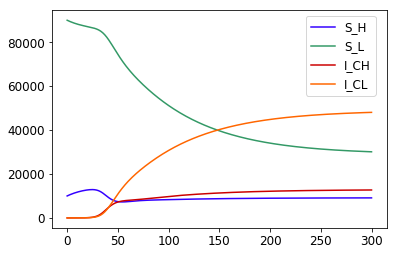
\includegraphics{im1}
		\caption{Динамика популяции по нерепрезентативным данным.}
	\end{figure}


	\begin{figure}[h!]
		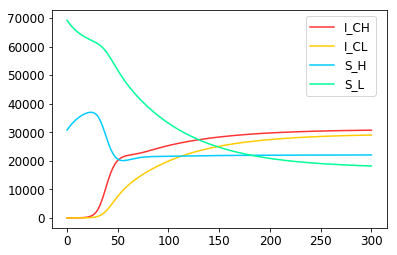
\includegraphics{im3}
		\caption{Реальная динамика популяции.}
	\end{figure}
	
	Графики на рисунке 4 отражают динамику популяции за 300 месяцев на основе нерепрезентативных данных, полученных в результате выборки в высокорисковой среде. 
	Зеленым и синим цветом выделены низкорисковые $S_L$ и высокорисковые $S_H$ здоровые индивиды соответственно, желтым и красным - низкорисковые $I_{CL}$ и высокорисковые $I_{CH}$ хронически инфицированные индивиды соответственно.
	
	На рисунке 5 показана искомая реальная динамика популяции. Зеленый, голубой, желтый и красный графики представляют $S_L$, $S_H$, $I_{CL}$ и $I_{CH}$ категории соответственно.
	
	\begin{figure}[h!]
	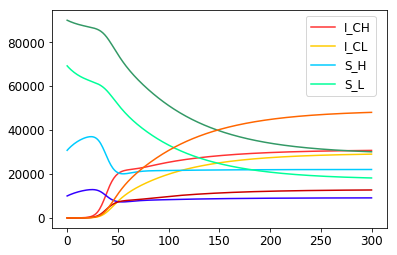
\includegraphics{im2}
	\caption{Сравнение результатов.}	
	\end{figure}

	Рисунок 6 демонстрирует существенную разницу в оценке популяции и ее развития до и после учета репрезентативности данных. Заметно снижение числа здоровых индивидов и рост числа инфицированных,придерживающихся высокорискового поведения. Стоит обратить внимание, что в общем число индивидов с высокорисковым поведением значительно больше, чем показывает тестирование и опросы. На основании чего можно сделать вывод о недостаточно высоком уровне жизни рассматриваемого населения.
	
	\begin{figure}[h!]
		\center{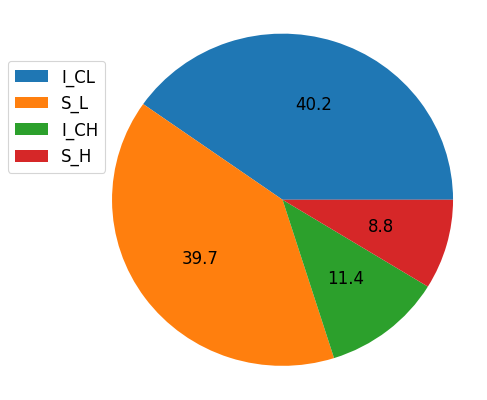
\includegraphics[scale=0.8]{im5}}
		\caption{Распределение населения по результатам тестирования, T = 150.}	
	\end{figure}
	
	\begin{figure}[h!]
		\center{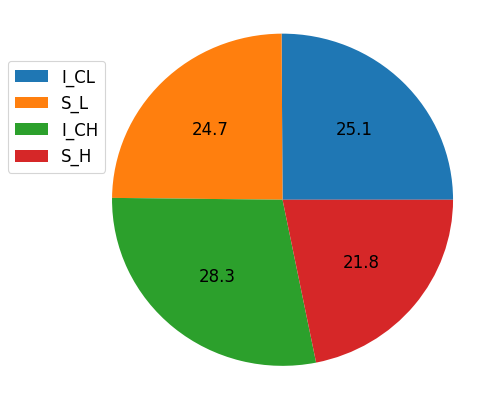
\includegraphics[scale=0.8]{im4}}
		\caption{Распределение населения после переоценки, T = 150.}	
	\end{figure}

	\newpage
	
	Рассмотрим, например, отношение долей в популяции по результатам тестирования (рисунок 7) и после их переоценки (рисунок 8). Очевидно, преобладание индивидов с низким уровнем риска ложно, тогда можно выдвинуть предположение о недостаточной пропаганде здорового образа жизни среди населения.

	\chapter*{Выводы}
	\addcontentsline{toc}{chapter}{\bfseries Выводы}

	Для решения поставленной задачи была разработана математическая модель, ее программная реализация, и численный эксперимент, проведенный на основе имеющихся данных о результатах опроса и тестирования. Такой эксперимент позволяет сравнить видение ситуации непосредственно на основе опросов и после переоценки долей с использованием формулы Байеса. Зная число людей после опроса и тестирования можно легко рассчитать соотношение таких категорий во всей популяции, указав результаты тестирования в абсолютных величинах, размер выборки и размер населения.
	
	Результаты эксперимента указывают на необходимость уделения повышенного внимания группе хронически инфицированных индивидов $I_{CH}$, рост которой был не так явно выражен до переоценки и коррекции данных.
	
	Сложностью исследования является невозможность распознавания острой фазы инфицирования при анонимном единовременном тестировании, искажающая реальную картину течения заболевания.	В будущем возможно более тщательное и подробное исследование, уделяющее особое внимание выявлению индивидов, находящихся в острой фазе инфицирования.
	
	Интересным продолжением работы может стать использование временных рядов для прогнозирования динамики популяции.	
		
		
	\chapter*{Заключение}
	\addcontentsline{toc}{chapter}{\bfseries Заключение}


	В ходе данной работы были достигнуты следующие результаты:
	
	Были проведен анализ различных существующих эпидемиологических моделей распространения инфекции.
	
	На основе этого была составлена математическая модель, представляющая популяцию как совокупность шести различных групп, учитывающая два уровня рискованного поведения и различные стадии инфицирования рассматриваемого населения: острая и хроническая.
	
	Приведен метод оценки соотношения категорий людей в выборке для нерепрезентативных данных, основываясь на их поведении, а затем вычисление долей в общей популяции для конкретного примера четырех состояний и для общего случая.
	
	Проанализированы коэффициенты модели, осуществлена программная реализация и проведен численный эксперимент для конкретной выборки.
	
	В дальшейшем приведенные методы и непосредственно программная реализация могут быть применены для составления плана лечения и профилактики населения. Это позволит прийти к решению, в какой мере инвестиции в предупреждающую и сдерживающую терапию должны быть увеличены в будущем для снижения уровня заболеваемости ВИЧ.
	
	Несмотря на глобальное развитие общества, ВИЧ остается экономически и социально значимым инфекционным заболеванием и актуальной проблемой для здравоохранения. Отсутствие на сегодняшний день достаточного количества  математических моделей, способных наиболее полно отразить особенности конкретного населения, подчеркивает актуальность проведенной работы.
	
	\chapter*{Список литературы}
	\addcontentsline{toc}{chapter}{\bfseries Список литературы}	
	\begin{thebibliography}{99}
		
		\bibitem{link1}
		WHO (2017) Global health observatory (GHO) data: HIV/AIDS. http://www.who.int/gho/hiv/en/ (last accessed 16 April 2018).
				
		\bibitem{link2}
		R. M. Anderson, R. M. May, and A. R. McLean, Possible demographic consequences of AIDS in developing countries, Nature (Land.) 332:228-234 (1988).
		
		\bibitem{link3}
		J. M. Hyman and E. A. Stanley, Using mathematical models to understand the AIDS epidemic, Math. Biosci. 90:415-474 (1988).
		
		\bibitem{link4}
		R. M. Anderson, S. P. Blythe, S. Gupta, and E. Konings. The transmission dynamics of the human immunodeficiency virus type 1 in the male homosexual community in the United Kingdom: the influence of changes in sexual behaviour, Phil. Trans. Roy. Sot. B 325:45-98 (1989).
		
		\bibitem{link5}
		R. M. Anderson, T. W. Ng, M. C. Boily, and R. M. May, The influence of different
		sexual contact patterns between age classes on the predicted demographic impacts of
		AIDS in developing countries, Ann. N.Y. Acad. Sci. 569:240-274 (1989). 
		
		\bibitem{link6}
		R. M. May and R. M. Anderson, The transmission dynamics of human immunodeficiency
		virus (HIV), Phil. Trans. Roy. Sot. B 321:565-607 (1989).
		
		\bibitem{link7}
		H. W. Hethcote, A model for HIV transmission and AIDS, in Mathematical Approaches to Problems in Resource Management and Epidemiology, Springer-Verlag, Berlin, 1989, eds. C. Castillo-Chavez, S. A. Levin, C. A. Shoemaker, pp. 164-176.
		
		\bibitem{link8}
		Hall H. I., Song R., Rhodes P., Prejean J., An Q., Lee L. M., Karon J., Brookmeyer R., Kaplan E. H., McKenna M. T. \& Janssen R. S. (2008) Estimation of HIV incidence in the United States. JAMA 300, 520–529.
		
		\bibitem{link9}
		Beyrer C., Baral S. D., Collins C., Richardson E. T., Sullivan P. S., Sanchez J., Trapence G., Katabira E., Kazatchkine M., Ryan O., Wirtz A. L. \& Mayer K. H. (2016) The global response to HIV in men who have sex with men. The Lancet 388, 198–206.
		
		\bibitem{link10}
		 Ю. Саранков. Медицинские потребности и проблемы мужчин, имеющих секс с мужчинами. // «СПИД Фонд Восток-Запад», 2006.
		
		\bibitem{link11}
		Paul Van de Ven, Pamela Rodden, June Crawford, Susan Kippax: A comparative demographic and sexual profile of older homosexually active men, Journal of Sex Research, 1997.
		
		\bibitem{link12}
		Данные «Объединённой программы ООН по ВИЧ/СПИДу». Декабрь 2006. http://www.unaids.org/ru.
		
		\bibitem{link13}
		СПИД и сексуальные отношения между мужчинами. Технический обзор, ЮНЭЙДС, 2000.
		
		\bibitem{link14}
		Diagnoses of HIV Infection in the United States and Dependent Areas. Surveillance Report, 2016.
		
		\bibitem{link15}
		С. Тюрин. Профилактика ВИЧ и ИППП среди МСМ. РОО «СПИД инфосвязь», 2007.

		\bibitem{link16}
		Gary De Young, Philip K. Main and Michael Nakamaye. Analysis of a Risk-Based Model for the Growth of AIDS Infection // Baltimore conference, August 1990
		
		\bibitem{link17}
		Jeremy M. G. Taylor. Models for the HIV infection and AIDS epidemic in the United States // Statistics in Medicine, 1989.
		
		\bibitem{link18}
		Punyacharoensin, N., Edmunds, W. J., De Angelis, D., White, R. G. Mathematical models for the study of HIV spread and control amongst men who have sex with men //
		Eur J Epidemiol, 2011.	
		
		\bibitem{link19}
		Punyacharoensin, N., Edmunds, W. J., De Angelis, D., White, R. G. Effect of pre-exposure prophylaxis and combination HIV prevention for men who have sex with men in the UK: a mathematical modelling study //  Lancet HIV, 2016.
		
		\bibitem{link20}
		Zhang X., Zhong L., Romero-Severson E., Alam S. J., Henry C. J., Volz E. M. \& Koopman J. S. (2012) Episodic HIV risk behavior can greatly amplify HIV prevalence and the fraction of transmissions from acute HIV infection. Stat. Commun. Infec. Dis. 4.
		
		\bibitem{link21}
		D. Gromov, I. Bulla, E. O. Romero-Severson, and O. S. Serea. Numerical optimal control for hiv prevention with dynamic budget allocation // Mathematical Medicine \& Biology, 2017.
		
		\bibitem{link22}
		D. Gromov, I. Bulla, E. O. Romero-Severson. Optimal Resource Allocation for HIV Prevention and Control // September 22, 2017
		
		\bibitem{link23}
		E. O. Romero-Severson, E. Volz, J. S. Koopman, T. Leitner, and E. L. Ion- ides. Dynamic variation in sexual contact rates in a cohort of HIV-negative gay men. American Journal of Epidemiology, 182(3):255–262, 2015.
		
		\bibitem{link24}
		S. E. Bellan, J. Dushoff, A. P. Galvani, and L. A. Meyers. Reassessment of HIV-1 acute phase infectivity: Accounting for heterogeneity and study design with simulated cohorts. PLoS Med, 12(3):e1001801, 2015.
		
	%	\bibitem{link25}	
		

	\end{thebibliography}



\chapter*{Приложение}
\addcontentsline{toc}{chapter}{\bfseries Приложение}

\section*{Приложение A. Описание модели и решение СОДУ.}


\lstset{language=Python}
\lstset{frame=lines}
\lstset{label={lst:code_direct}}
\lstset{basicstyle=\ttfamily}
%\lstset{basicstyle=\footnotesize}
\lstset{commentstyle=\color{blue}, }

\begin{lstlisting}

# coding: utf-8
import pandas as pd
import numpy as np
from scipy import integrate
import matplotlib.pyplot as plt

# known coefficients of the model
mu = 1 / (12 * 30)
delta_A = 1 / 4
delta_C = 1 / 116
x = 1 / 12
y = 0
r_b = 0.8 / 0.2
lambda_H = 43.478;
lambda_L = 5.4896
beta_A = 0.015;
beta_C = 0.001
rho_H = 0.041667;
rho_L = 0.0046296
pi = 0.5


# HIV-model
def HIV(t, X):
	# a column vector
	dX = np.zeros((len(X), 1)) 
	
	# state variables
	# S_H = X(1)
	# S_L = X(2)
	# I_AH = X(3)
	# I_AL = X(4)
	# I_CH = X(5)
	# I_CL = X(6)
	S_H, S_L, I_AH, I_AL, I_CH, I_CL = X
	
	# auxiliary variables
	N_H = S_H + I_AH + I_CH
	N_L = S_L + I_AL + I_CL
	N = N_H + N_L
	
	# calculated coefficients of the model
	alpha = mu * N + delta_C * (I_CH + I_CL)
	alpha_H = 0.9 * alpha
	alpha_L = 0.1 * alpha
	
	theta = lambda_H * N_H + lambda_L * N_L

	sigma = (beta_A * (lambda_H * I_AH \
			 + lambda_L * I_AL) \
	       + beta_C * (lambda_H * I_CH \
   			 + lambda_L * I_CL)) / theta
	
	psi_H = pi * lambda_H * (beta_A * I_AH / N_H \
		               + beta_C * I_CH / N_H)
	psi_L = pi * lambda_L * (beta_A * I_AL / N_L \
		               + beta_C * I_CL / N_L)
	
	tau_H = (1 - pi) * lambda_H * sigma
	tau_L = (1 - pi) * lambda_L * sigma
	
	phi_H = psi_H + tau_H
	phi_L = psi_L + tau_L
	
	# ODE
	dS_H = alpha_H \
	     - (phi_H + rho_H + mu) * S_H \
	     + rho_L * S_L
	     
	dS_L = alpha_L \
	     - (phi_L + rho_L + mu) * S_L \
	     + rho_H * S_H
	
	dI_AH = phi_H * S_H \
	      - (rho_H + mu + delta_A) * I_AH \
	      + rho_L * I_AL
	     
	dI_AL = phi_L * S_L \
	      - (rho_L + mu + delta_A) * I_AL \
	      + rho_H * I_AH
	
	dI_CH = delta_A * I_AH \
	      - (rho_H + mu + delta_C) * I_CH \
	      + rho_L * I_CL
		
	dI_CL = delta_A * I_AL \
	      - (rho_L + mu + delta_C) * I_CL \
	      + rho_H * I_CH
	
	dX = np.array(
	[dS_H, dS_L, dI_AH, dI_AL, dI_CH, dI_CL]
	)
	return dX

# ODE solution
r = integrate.ode(HIV).set_integrator(
	"dopri5",
	atol=1e-8,
	rtol=1e-4,
)

# 300 months interval
X0 = np.array([10000, 89998, 1, 1, 0, 0])
T0 = 0
T1 = 300
dt = 1
X = []
# [0 300], 300 points
# for step = 1
t = np.array(list((i for i in range(T0, T1 + 1))))
r.set_initial_value(X0, T0)
for ti in t:
	X.append(r.integrate(ti))
T = np.array(t)
X = np.array(X)
data = pd.DataFrame(
X,
columns=['S_H', 'S_L', 'I_AH', 'I_AL', 'I_CH', 'I_CL'],
)
data['T'] = T

# the states are:
# S_H, S_L -- high- and low-risk susceptibles,
# I_AH,I_AL -- high- and low-risk infected in acute phase,
# we add S_H and I_AH (and the same for S_L and I_AL)
# as we cannot distinguish them,
# finally I_CH, I_CL -- high- and low-risk infected in
				# chronical phase.

# ODE fractions plots
plt.plot(T, data.S_H.values + data.I_AH.values, \
		'#3300FF', label='S_H')
plt.plot(T, data.S_L.values + data.I_AL.values, \
		'#339966', label='S_L')
plt.plot(T, data.I_CH.values, \
		'#CC0000', label='I_CH')
plt.plot(T, data.I_CL.values, \
		'#FF6600', label='I_CL')
\end{lstlisting}

\newpage
\section*{Приложение B. Оценка долей в популяции.}

\begin{lstlisting}

# number of all high-risk people
N_H = data.S_H + data.I_AH + data.I_CH
# number of all low-risk people
N_L = data.S_L + data.I_AL + data.I_CL
N = N_H + N_L

# computing the corrected fractions
# high-risk susceptibles
F_SH = (r_b * data.S_H) \
	.divide(r_b * N_H + N_L) \
	.multiply(N) \
     + (r_b * data.I_AH) \
	.divide(r_b * N_H + N_L) \
	.multiply(N)
# low-risk susceptibles
F_SL = data.S_L \
	.divide(r_b * N_H + N_L) \
	.multiply(N) \
     + data.I_AL \
	.divide(r_b * N_H + N_L) \
	.multiply(N)
# high-risk infected
F_ICH = r_b * data.I_CH \
	.divide(r_b * N_H + N_L) \
	.multiply(N)
# low-risk infected
F_ICL = data.I_CL \
	.divide(r_b * N_H + N_L) \
	.multiply(N)
	
data2 = pd.DataFrame(
np.array([F_SH, F_SL, F_ICH, F_ICL]).transpose(),
columns=['F_SH', 'F_SL', 'F_ICH', 'F_ICL']
)

# given fractions plots
plt.plot(T, data.S_H.values + data.I_AH.values, \
		'#3300FF', label='S_H')
plt.plot(T, data.S_L.values + data.I_AL.values, \
		'#339966', label='S_L')
plt.plot(T, data.I_CH.values, \
		'#CC0000', label='I_CH')
plt.plot(T, data.I_CL.values, \
		'#FF6600', label='I_CL')

# Bayes-corrected fractions plots
plt.plot(T, data2.F_ICH.values, \
		'#FF3333', label='F_ICH')
plt.plot(T, data2.F_ICL.values, \
		'#FFCC00', label='F_ICL')
plt.plot(T, data2.F_SH.values, \
		'#00CCFF', label='F_SH')
plt.plot(T, data2.F_SL.values, \
		'#00FF99', label='F_SL')
\end{lstlisting}

\newpage
\section*{Приложение C. Оценка количества людей в различных состояниях.}

\begin{lstlisting}
# matrix with r_b coefficiets calculation
RB = pd.DataFrame(
	np.array([
		np.array([r_b, 0, 0]),
		np.array([0, r_b, 0]),
		np.array([0, 0, 1]),
	]),
	index=['0', '1', '2'],
)

ANS = []
for i in range(0, 301):
	F = np.array([
		    F_SH[i],
		    F_ICH[i],
		    F_ICL[i]
	]) / 100000
	# diagonal matrix calculation
	DG = pd.DataFrame(np.array([
		np.array([F_SH[i], 0, 0]),
		np.array([0, F_ICH[i], 0]),
		np.array([0, 0, F_ICL[i]]),
	])) / 100000
	# 1 and 0 matrix calculation
	SMTH = pd.DataFrame(
		np.array([
			np.array([1, 1, 0]),
			np.array([1, 1, 0]),
			np.array([1, 1, 0]),
		])
	)
	SMTH2 = ((1 - r_b) * DG).dot(SMTH)
	COEF = RB + SMTH2.values
	ans = list(np.linalg.pinv(COEF.values).dot(F))
	# the last fraction calculation
	# 1 - sum of others
	ans.insert(1, 1 - sum(ans))
	ANS.append(pd.Series(ans))
ANS = pd.DataFrame(
	ANS,
#     columns=['S_H', 'S_L', 'I_CH', 'I_CL'],
)
ANS = ANS.rename(
	columns={
		0: 'A',
		1: 'B',
		2: 'C',
		3: 'D',
	},
)
plt.plot(T, data.S_H.values + data.I_AH.values, \
		'#3300FF', label='S_H')
plt.plot(T, data.S_L.values + data.I_AL.values, \
		'#339966', label='S_L')
plt.plot(T, data.I_CH.values, \
		'#CC0000', label='I_CH')
plt.plot(T, data.I_CL.values, \
		'#FF6600', label='I_CL')
\end{lstlisting}


\newpage
\section*{Приложение D. Построение диаграммы.}

\begin{lstlisting}
import matplotlib as mpl
import matplotlib.pyplot as plt
import matplotlib.dates as mdates
import datetime as dt
import csv

data_names = ['I_CL', 'S_L', 'I_CH', 'S_H']
data_values = [
	data2.F_ICL[150],
	data2.F_SL[150],
	data2.F_ICH[150],
	data2.F_SH[150],
	]

dpi = 80
fig = plt.figure(
	dpi = dpi,
	figsize = (500 / dpi, 500 / dpi)
	)
mpl.rcParams.update({'font.size': 9})

plt.title('Population distribution')

xs = range(len(data_names))

plt.pie(data_values, autopct='%.1f', radius = 1.1)
plt.legend(
	bbox_to_anchor = (-0.16, 0.45, 0.25, 0.25),
	loc = 'lower left',
	labels = data_names
	)

\end{lstlisting}



\end{document}